\documentclass{article}
\usepackage[utf8]{inputenc}
\usepackage{setspace}
\usepackage{tikz}
\usetikzlibrary{positioning}
\usepackage{amsfonts}
\usepackage{amssymb}
\usepackage{amsmath}
\usepackage{amsthm}
\usepackage{systeme}
\usepackage{mathtools}
\usepackage{hyperref}
\usepackage{venndiagram}
\usepackage{pgfplots}
\usetikzlibrary{pgfplots.statistics}
\pgfplotsset{compat=newest}
\usepackage{logicproof}
\usepackage{mathrsfs}
\allowdisplaybreaks
\usepackage{mathpartir}
\usepackage{graphicx}

\begin{document}

\section*{Book}

~

Reimer, D. W. (2014). Count like an egyptian : A hands-on introduction to ancient mathematics. Princeton University Press.

\newpage

\section*{Question 1}

~

\subsection*{a}

~

\begin{align*}
    &18=16+2\\
    &1\times25=25\\
    &2\times25=50/\\
    &4\times25=100\\
    &8\times25=200\\
    &16\times25=400/\\
    &16\times25+2\times25=400+50=450\\
    \Rightarrow&18\times25=450\\
\end{align*}

~

\subsection*{b}

~

\begin{align*}
    &105=64+32+8+1\\
    &1\times59=59/\\
    &2\times59=118\\
    &4\times59=236\\
    &8\times59=472/\\
    &16\times59=944\\
    &32\times59=1888/\\
    &64\times59=3776/\\
    &1\times59+8\times59+32\times59+64\times59=59+472+1888+3776=6195\\
    \Rightarrow&105\times59=6195\\
\end{align*}

\newpage

\section*{Question 2}

~

\subsection*{a}
~
\begin{center}
\begin{tabular}{ccc}
        8 &  1&/\\
        16 & 2&/\\
        32&4&/\\
        64&8\\
        128&16&/\\
\end{tabular}
\end{center}
\[
\Rightarrow 184/8=1+2+4+16=23\\
\]

~

\subsection*{b}

~

\begin{center}
\begin{tabular}{ccc}
        9&  1&/\\
        18 & 2&\\
        36&4&/\\
\end{tabular}
\end{center}

\begin{align*}
    &47-(1\times9+4\times9)=2\\
    \Rightarrow&\frac{47}{9}=5+\frac{2}{9}\\
    &\frac{2}{9}=\frac{1}{6}+\frac{1}{18}(\text{by Rhind Papyrus})\\
    \Rightarrow&\frac{47}{9}=5\frac{1}{6}\frac{1}{18}\\
\end{align*}

~

\subsection*{c}

~

\begin{center}
\begin{tabular}{ccc}
    1& 51& \\
    $\frac{2}{3}$&34&1$\frac{1}{2}$\\
    $2$&102&$\frac{1}{2}$\\
\end{tabular}
\end{center}
\[\Rightarrow \frac{2}{51}=\frac{1}{34}\frac{1}{102}
\]

\begin{center}
\begin{tabular}{ccc}
    1& 99& \\
    $\frac{2}{3}$&66&1$\frac{1}{2}$\\
    $2$&198&$\frac{1}{2}$\\
\end{tabular}
\end{center}
\[\Rightarrow \frac{2}{99}=\frac{1}{66}\frac{1}{198}
\]

\newpage

\section*{Question 3}

~

\[ 140\div(2\times 93\frac{1}{3})=140\div(186\frac{2}{3})
\]

\begin{center}
    \begin{tabular}{ccc}
        1 & $186\frac{2}{3}$&\\
        $\frac{3}{280}$ & 2&$93\frac{1}{3}$\\
        $\frac{3}{140}$&4&$46\frac{1}{2}\frac{1}{6}$\\
    \end{tabular}
\end{center}

\begin{align*}
    \Rightarrow&\frac{140}{186\frac{2}{3}}=\frac{1}{2}\frac{1}{4}\\
    &\frac{1}{2}\frac{1}{4}\times7\\
    &7=1+2+4\\
\end{align*}

\begin{center}
    \begin{tabular}{ccc}
        $\frac{1}{2}$&1&/  \\
        1&2&/\\
        2&4&/\\
    \end{tabular}
\end{center}

\begin{center}
    \begin{tabular}{ccc}
        $\frac{1}{4}$&1&/  \\
        $\frac{1}{2}$&2&/\\
        1&4&/\\
    \end{tabular}
\end{center}

\begin{align*}
    \Rightarrow&\frac{1}{2}\times7=3\frac{1}{2}\\
    \Rightarrow&\frac{1}{4}\times7=1\frac{1}{2}\frac{1}{4}\\
    &\frac{1}{2}\frac{1}{4}\times7=3\frac{1}{2}+1\frac{1}{2}\frac{1}{4}=5\frac{1}{4}\\
    &4=4\\
\end{align*}

\begin{center}
    \begin{tabular}{ccc}
        $\frac{1}{4}$ & 1 &\\
        $\frac{1}{2}$ & 2&\\
        1&4&/\\
    \end{tabular}
\end{center}

\[
\Rightarrow\frac{1}{4}\times4=1\\
\]

\[
\Rightarrow 5\text{ palms }1\text{ finger}
\]

\newpage

\section*{Question 4}

~

\begin{align*}
    &a=7\\
    &a_1=2.5\\
    &b_1=\frac{a}{a_1}=\frac{14}{5}\\
    &a_2=\frac{1}{2}(a_1+b_1)=2.65\\
    &b_2=\frac{a}{a_2}=\frac{7}{2.65}\\
    &a_3=\frac{1}{2}(a_2+b_2)=\frac{5609}{2120}\approx2.64575\\
    &\sqrt{7}\approx2.64575\\
    &\text{Using two steps to get the estimation }a_3\approx2.64575\\
\end{align*}

\newpage

\section*{Question 5}

~

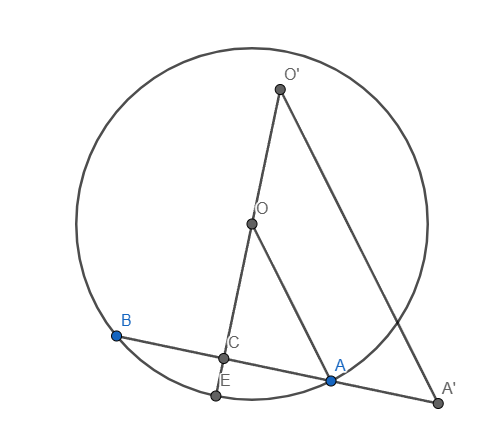
\includegraphics[scale=0.8]{HW_0207/HW_0207.png}

By the figure, $AB$ is a chord of the circle $O$, and $OE$ is a radius perpendicular to $AB$ and intersects at $C$. By the inscription, circumference is 60, by $C=2\pi r$ and $\pi=3$, $r=10$. So $OE=10$, and $CE$, which is the sagitta, is 2. $OC=OC-CE=8$. And extending $O$ to $O'$ so that $OC=O'O=\frac{1}{2}O'C$, extending $A$ to $A'$ so that $AC=A'A=\frac{1}{2}A'C$, the two triangles, $\Delta A'CO'$ and $ACO$ are similar triangles, so $AO$ and $A'O'$ should have the same ratio as others, which is $A'O'=2AO$, $AO$ is the radius, which is 10, so $A'O'=20$. $O'C=2OC=16$. So by the Pythagorean theorem, $A'C=\sqrt{{A'O'}^2-{O'C}^2}=12$, and since AB is a chord and $OC$ is perpendicular and goes through the center, $C$ bisects $AB$, so $AC=\frac{1}{2}AB$, also $AC=\frac{1}{2}A'C$, so $AB=A'C$. As calculated by the Pythagorean theorem before, $A'C=12$, so $AB=12$. So the calculation in the inscription is true.
\end{document}